\documentclass[../thesis.tex]{subfiles}
\begin{document}
\chapter{System design and implementation}\label{cap:system-design-and-implementation}
The system is composed of two components: a node that deals with  hand gesture recognition and a node representing the robot to be controlled. The tasks that the robot must perform are:
\begin{itemize}
    \item Pick up a parcel;
    \item Drop down a parcel;
    \item Go to a predetermined position.
\end{itemize}
A letter identified positions and parcels. In this way, the \glsfirst{ASL} is exploitable in order to simulate the identification of positions and parcels.\\
Starting from these assumptions a finite state automataton can be used to check the correctness of the input. Figure~\ref{fig:automata_for_commands} shows the transition diagram for a possible automataton with this purpose. The alphabet is $\Sigma = \{[A-Z], go\, to, pick\, up, drop\, down\}$ and the states are:
\begin{itemize}
    \item \textbf{$q_0$}: robot without parcel; 
    \item \textbf{$q_1$}: robot waiting for parcel id; 
    \item \textbf{$q_2$}: robot waiting for a ``direction'' without a parcel;
    \item \textbf{$q_3$}: robot with a parcel;
    \item \textbf{$q_4$}: robot waiting for a ``direction'' with a parcel.
\end{itemize}

\begin{figure}[H]
    \centering
    \resizebox{0.8\textwidth}{!}{%
    \begin{tikzpicture}[node distance = 4cm, on grid]
        \node (q0) [state, initial, accepting] {$q_0$};
        \node (q1) [state, above right = of q0] {$q_1$};
        \node (q3) [state, right = of q1] {$q_3$};
        \node (q4) [state, below right = of q3] {$q_4$};
        \node (q2) [state, below right = of q0] {$q_2$};

        \path [-stealth, thick]
            (q0) edge node[below right] {pick up} (q1)
            (q1) edge node[auto] {[A-Z]} (q3)
            (q3) edge node[auto] {go to} (q4)
            (q4) edge [bend left, auto] node {[A-Z]} (q3)
            (q0) edge node[auto] {go to} (q2)
            (q2) edge [bend left, auto] node {[A-Z]} (q0)
            (q3) edge [in=90,out=120,above,distance=3cm, auto] node[above left] {drop down} (q0);
    \end{tikzpicture}%
}
    \caption{Automata diagram for commands.}\label{fig:automata_for_commands}
\end{figure}
\gls{ROS} and its communication layer (i.e. exchange of messages) have to be used for the node implementation in order to comply with the requirement of interoperability between robots. For this reason, the hand gesture recognizer must be encapsulated inside a \gls{ROS} node.

\section{Hand gesture recognizer}
Two types of hand gestures have been considered:
\begin{itemize}
    \item \textbf{Static hand gestures}: in which the hand doesn't move and only a snapshot of the position of the fingers is sufficient to recognize the gesture;
    \item \textbf{Dynamic hand gesture}: in which the hand performs a movement. In this case, a sequence of data is necessary to recognize the gesture. 
\end{itemize}
This diversity leads to two different neural networks to classify the hand gesture the user is doing.\\
The hand gesture recognizer has been developed starting from the project of~\citeauthor{site:hand_gesture_base_repo}~\cite{site:hand_gesture_base_repo} to which several improvements have been made. Figure~\ref{fig:interface} shows the user interface of the hand gesture recognizer. In which, the following components are recognizable:
\begin{itemize}
    \item the hand tracker's landmarks: the black dots inside the green rectangle;
    \item the history of landmarks to recognize dynamic gestures: the green dots inside the green rectangle;
    \item the recognized static hand gesture: the letter inside the orange rectangle;
    \item the recognized dynamic hand gesture: the word inside the pink rectangle;
    \item the number of frame per seconds: the number inside the red rectangle.
\end{itemize}

\begin{figure}[H]
    \centering
    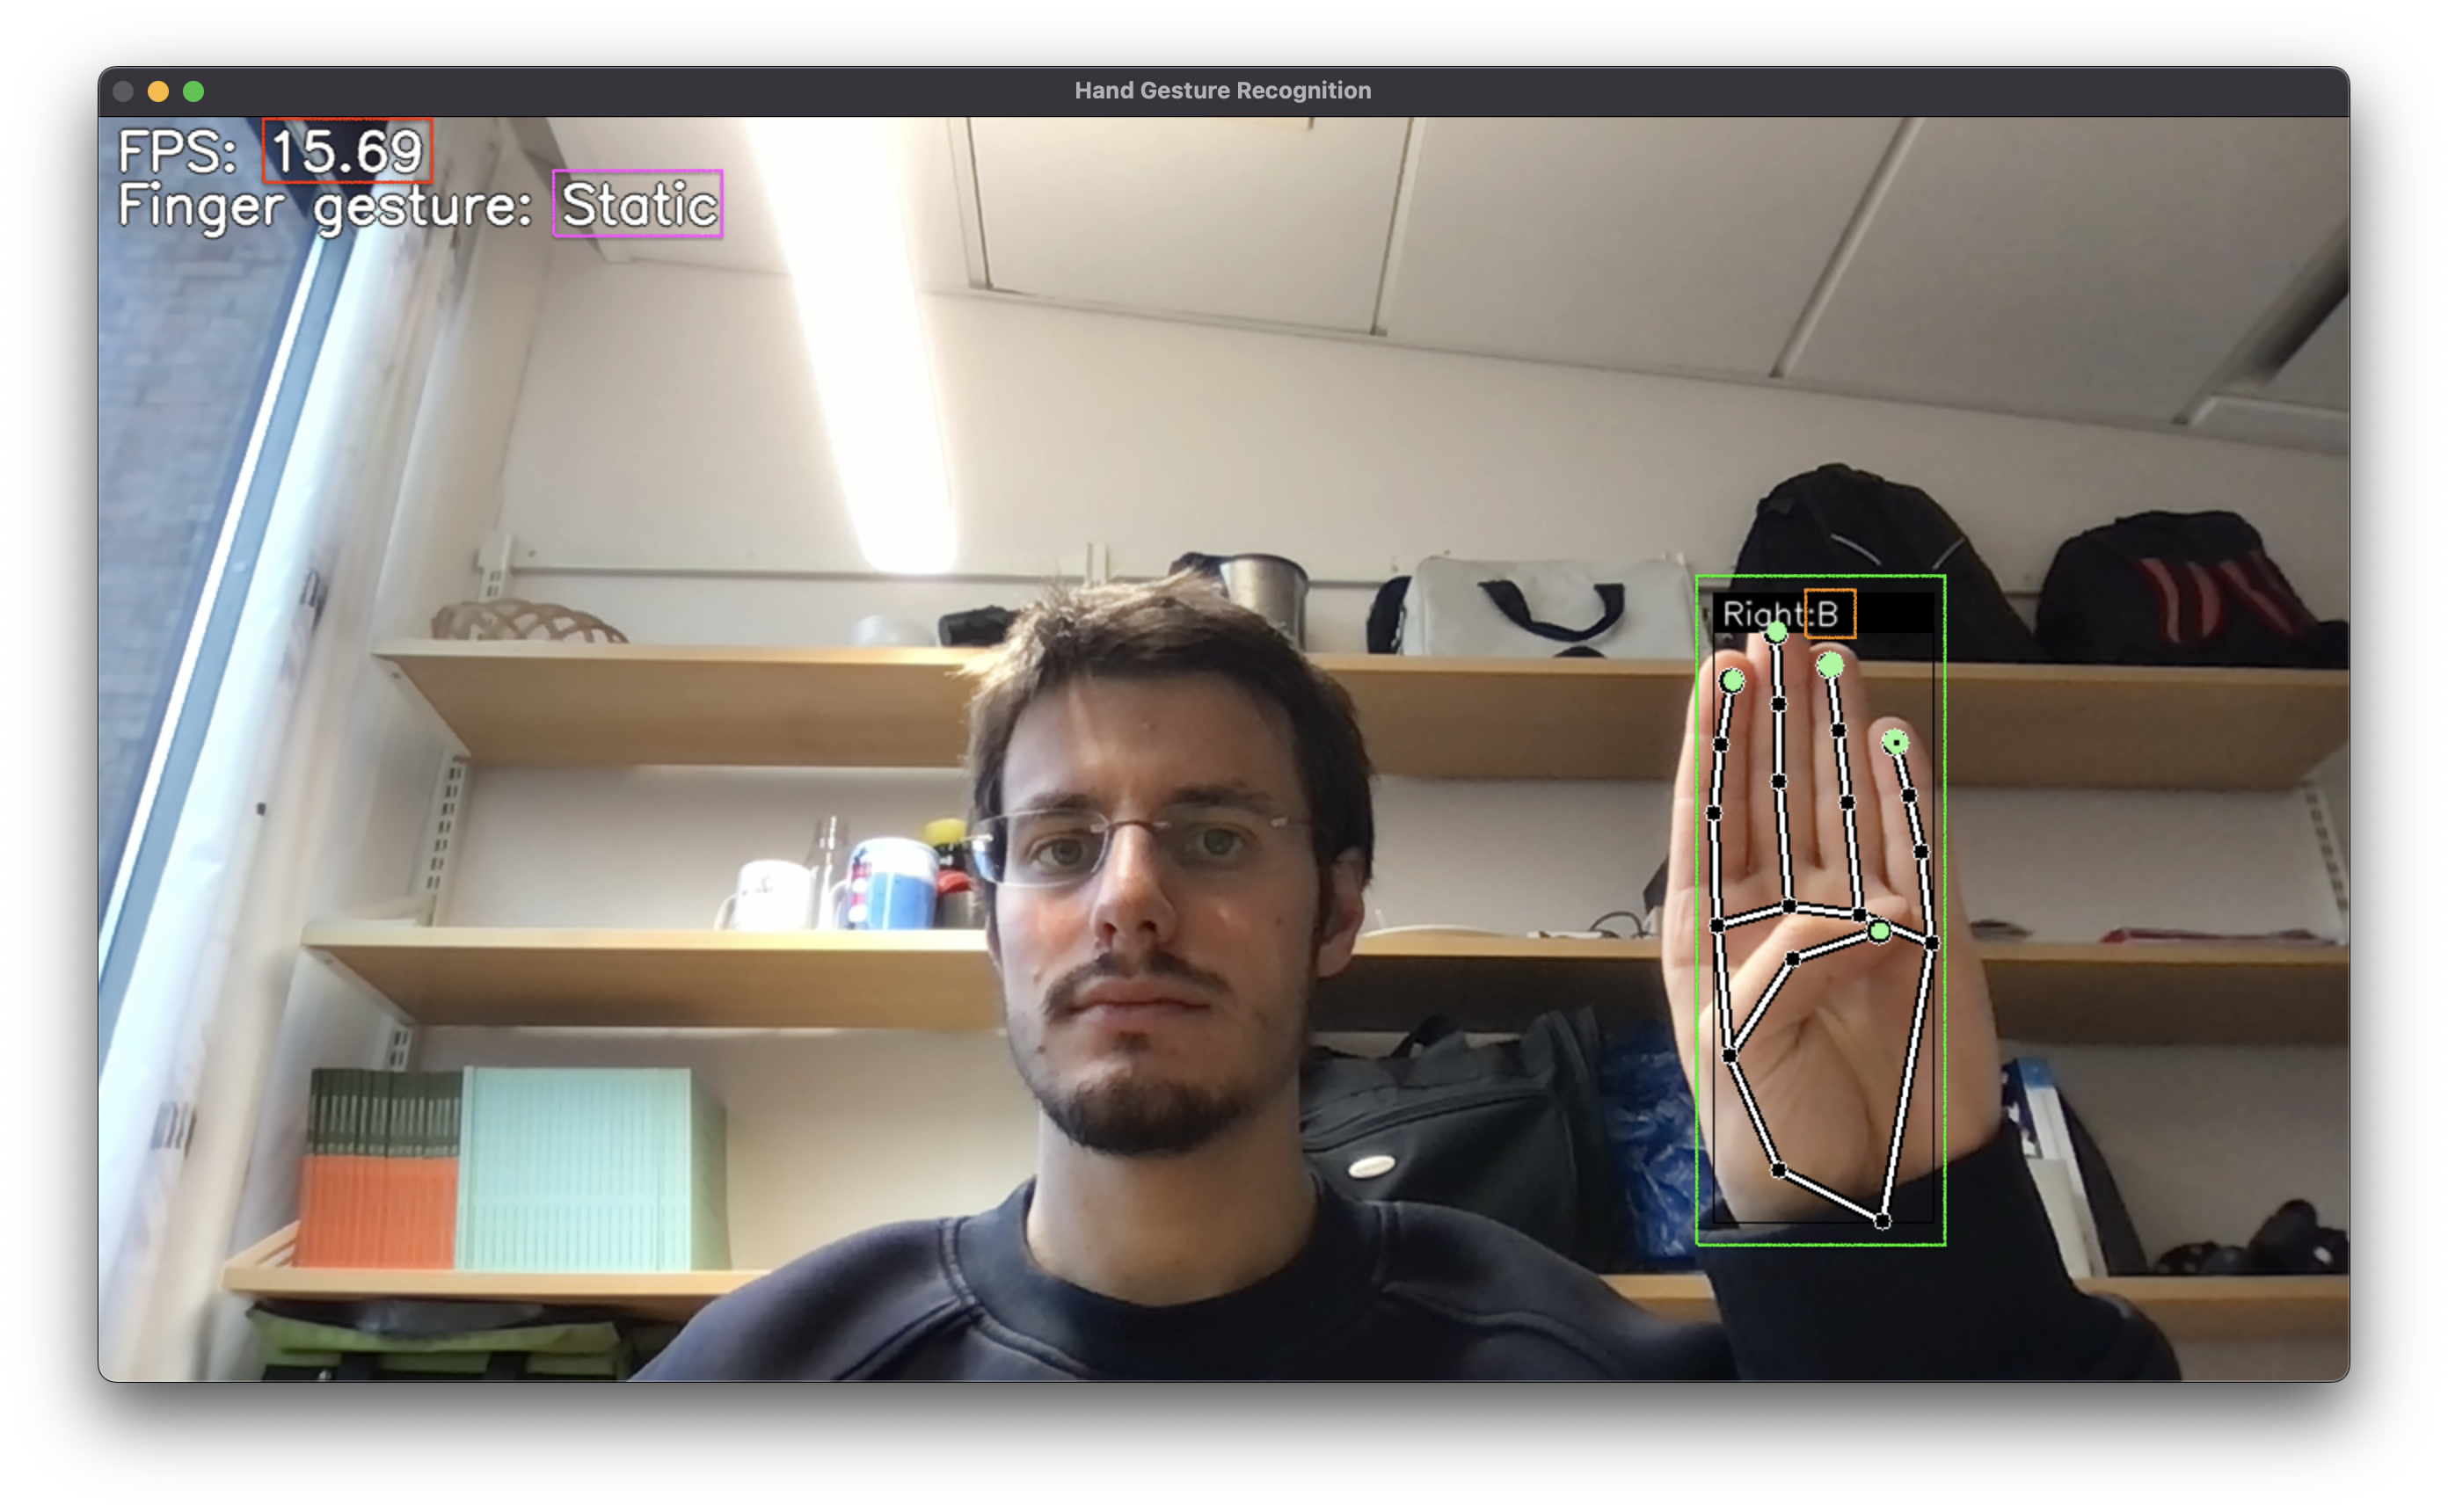
\includegraphics[width=\textwidth]{example_interface.png}
    \caption{User interface of the hand gesture recognizer.}\label{fig:interface}
\end{figure}

\subsection{Static hand gestures}
The set of static hand gestures chosen is the \gls{ASL} (in figure~\ref{fig:asl}), \textit{J} \textit{Z} excluded because they involve a movement. To discriminate between dynamic and static gestures, I decided to prioritize the dynamic ones because the user has to perform an action to activate them. Instead, with the static gestures, the hand doesn't move, and the recognizer will always return a prediction. Also the numbers have been excluded.

\begin{figure}
    \centering
    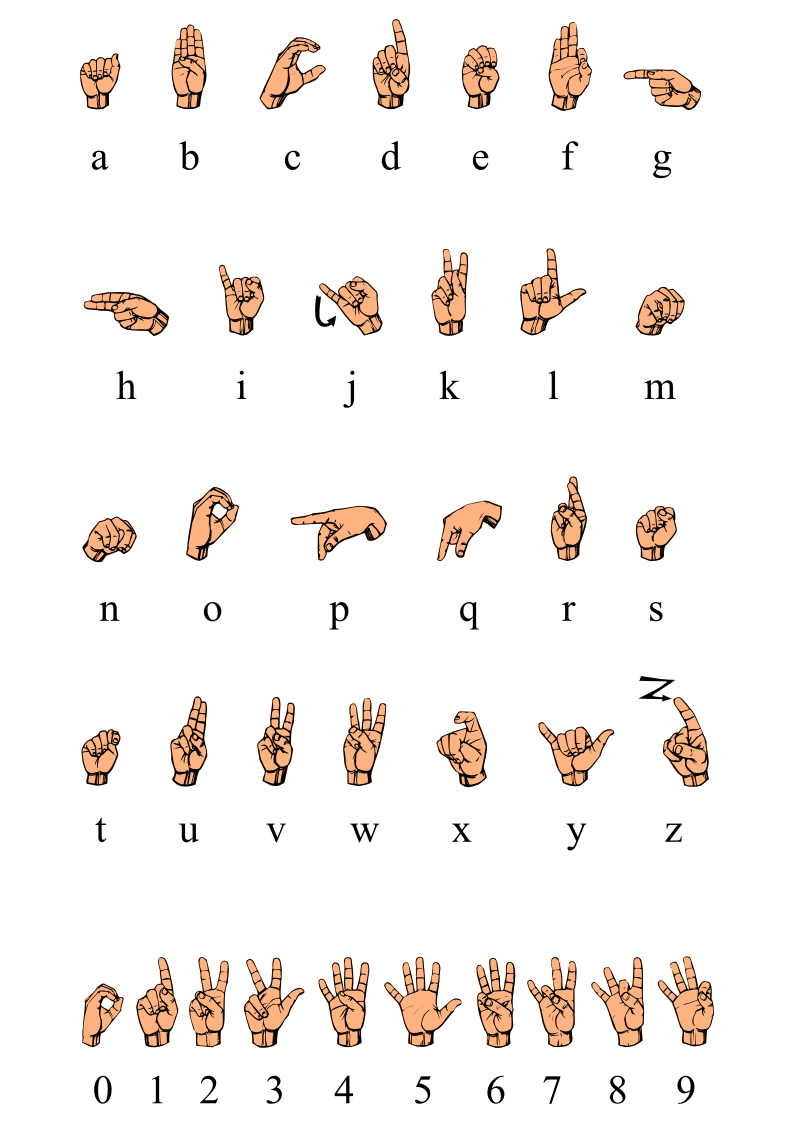
\includegraphics[width=\textwidth]{asl.png}
    \caption{\glsdesc{ASL}~\parencite{img:asl}}\label{fig:asl}
\end{figure}

\subsubsection{MediaPipe data}

\subsubsection{Deep neural network}

\subsubsection{Training}

\subsection{Dynamic hand gestures}

\subsubsection{MediaPipe data}

\subsubsection{Deep neural network}

\subsubsection{Training}

\section{Integration with ROS}

\end{document}
